\documentclass[10pt,a4paper]{article}
\usepackage[margin=2.2cm]{geometry}
\usepackage[T1]{fontenc}
\usepackage{lmodern}
\usepackage{microtype}
\usepackage{amsmath,amssymb}
\usepackage{graphicx}
\usepackage{booktabs}
\usepackage{caption}
\usepackage{xcolor}
\usepackage{enumitem}
\usepackage[section]{placeins}
\usepackage[colorlinks=true,linkcolor=blue!50!black,urlcolor=blue!50!black,citecolor=blue!50!black]{hyperref}
\captionsetup{font=small,labelfont=bf}
\setlist{itemsep=2pt,topsep=3pt}
\graphicspath{{figures/}}
% numbers quoted in the text (written by analyse.py)
\newcommand{\GeoDefIncMed}{+1.3}
\newcommand{\GeoDefIncSig}{6.2}
\newcommand{\GeoDefPASig}{2.0}
\newcommand{\GeoDefVSig}{9}
\newcommand{\GeoDefVMed}{\ensuremath{-}4.7}
\newcommand{\GeoDefWithin}{50}
\newcommand{\GeoDefMove}{3.3}
\newcommand{\GeoDefCorr}{0.90}
\newcommand{\GeoDefInitSig}{5.5}
\newcommand{\GeoDefInitMed}{+2.7}
\newcommand{\GeoWideIncMed}{+1.6}
\newcommand{\GeoWideIncSig}{7.4}
\newcommand{\GeoWidePASig}{2.3}
\newcommand{\GeoWideVSig}{10}
\newcommand{\GeoWideVMed}{\ensuremath{-}4.5}
\newcommand{\GeoWideWithin}{38}
\newcommand{\GeoWideMove}{3.9}
\newcommand{\GeoWideCorr}{0.81}
\newcommand{\GeoWideInitSig}{5.5}
\newcommand{\GeoWideInitMed}{+2.7}
\newcommand{\GeoTrueIncMed}{+1.8}
\newcommand{\GeoTrueIncSig}{3.3}
\newcommand{\GeoTruePASig}{1.7}
\newcommand{\GeoTrueVSig}{6}
\newcommand{\GeoTrueVMed}{\ensuremath{-}3.9}
\newcommand{\GeoTrueWithin}{43}
\newcommand{\GeoTrueMove}{3.3}
\newcommand{\GeoTrueCorr}{\ensuremath{-}0.00}
\newcommand{\GeoTrueInitSig}{0.0}
\newcommand{\GeoTrueInitMed}{+0.0}
\newcommand{\WarpDefIncMed}{+0.0}
\newcommand{\WarpDefIncSig}{5.0}
\newcommand{\WarpDefPASig}{1.8}
\newcommand{\WarpDefVSig}{3}
\newcommand{\WarpDefVMed}{\ensuremath{-}1.9}
\newcommand{\WarpDefWithin}{40}
\newcommand{\WarpDefMove}{3.1}
\newcommand{\WarpDefCorr}{0.92}
\newcommand{\WarpDefInitSig}{7.3}
\newcommand{\WarpDefInitMed}{+1.5}
\newcommand{\WarpWideIncMed}{+0.2}
\newcommand{\WarpWideIncSig}{4.3}
\newcommand{\WarpWidePASig}{1.9}
\newcommand{\WarpWideVSig}{3}
\newcommand{\WarpWideVMed}{\ensuremath{-}0.9}
\newcommand{\WarpWideWithin}{54}
\newcommand{\WarpWideMove}{3.6}
\newcommand{\WarpWideCorr}{0.83}
\newcommand{\WarpWideInitSig}{7.3}
\newcommand{\WarpWideInitMed}{+1.5}
\newcommand{\WarpTrueIncMed}{\ensuremath{-}0.3}
\newcommand{\WarpTrueIncSig}{2.0}
\newcommand{\WarpTruePASig}{1.8}
\newcommand{\WarpTrueVSig}{2}
\newcommand{\WarpTrueVMed}{\ensuremath{-}1.1}
\newcommand{\WarpTrueWithin}{88}
\newcommand{\WarpTrueMove}{1.3}
\newcommand{\WarpTrueCorr}{\ensuremath{-}0.06}
\newcommand{\WarpTrueInitSig}{0.0}
\newcommand{\WarpTrueInitMed}{+0.0}
\newcommand{\WarpDefIncSlope}{\ensuremath{-}0.02}
\newcommand{\WarpDefPASlope}{0.58}
\newcommand{\WarpDefIncRes}{9.7}
\newcommand{\WarpDefPARes}{10.2}
\newcommand{\WarpWideIncSlope}{\ensuremath{-}0.19}
\newcommand{\WarpWidePASlope}{0.54}
\newcommand{\WarpWideIncRes}{12.2}
\newcommand{\WarpWidePARes}{11.2}
\newcommand{\WarpTrueIncSlope}{0.68}
\newcommand{\WarpTruePASlope}{0.77}
\newcommand{\WarpTrueIncRes}{4.5}
\newcommand{\WarpTruePARes}{7.1}
\newcommand{\CppGeoN}{200}
\newcommand{\CppGeoDiff}{0.9}
\newcommand{\CppGeoCorr}{0.89}
\newcommand{\CppN}{672}
\newcommand{\CppVSig}{2.0}
\newcommand{\CppVMed}{\ensuremath{-}0.1}
\newcommand{\CppSSig}{13.6}
\newcommand{\CppSMed}{\ensuremath{-}0.4}
\newcommand{\CppVpySig}{4.0}
\newcommand{\CppVcppSig}{4.2}
\newcommand{\CppSpyMed}{+1}
\newcommand{\CppScppMed}{+2}
\newcommand{\MaskSearchFiveS}{\ensuremath{-}50.3}
\newcommand{\MaskSearchFiveV}{\ensuremath{-}5.2}
\newcommand{\MaskSearchFiveInc}{+4.8}
\newcommand{\MaskSearchTenS}{\ensuremath{-}12.3}
\newcommand{\MaskSearchTenV}{\ensuremath{-}2.3}
\newcommand{\MaskSearchTenInc}{+3.4}
\newcommand{\MaskSearchTwentyS}{+4.1}
\newcommand{\MaskSearchTwentyV}{\ensuremath{-}1.6}
\newcommand{\MaskSearchTwentyInc}{+0.3}
\newcommand{\MaskSearchFortyS}{+7.0}
\newcommand{\MaskSearchFortyV}{\ensuremath{-}0.6}
\newcommand{\MaskSearchFortyInc}{\ensuremath{-}3.1}
\newcommand{\MaskSmoothFiveS}{\ensuremath{-}30.9}
\newcommand{\MaskSmoothFiveV}{\ensuremath{-}3.9}
\newcommand{\MaskSmoothFiveInc}{+4.6}
\newcommand{\MaskSmoothTenS}{\ensuremath{-}8.6}
\newcommand{\MaskSmoothTenV}{\ensuremath{-}2.2}
\newcommand{\MaskSmoothTenInc}{+1.1}
\newcommand{\MaskSmoothTwentyS}{+1.9}
\newcommand{\MaskSmoothTwentyV}{\ensuremath{-}0.9}
\newcommand{\MaskSmoothTwentyInc}{\ensuremath{-}1.1}
\newcommand{\MaskSmoothFortyS}{+4.1}
\newcommand{\MaskSmoothFortyV}{\ensuremath{-}0.1}
\newcommand{\MaskSmoothFortyInc}{\ensuremath{-}3.7}
\newcommand{\MaskNoneFiveS}{+737}
\newcommand{\MaskNoneFiveV}{\ensuremath{-}1.0}
\newcommand{\MaskNoneFiveInc}{+0.4}
\newcommand{\MaskNoneTenS}{+69.4}
\newcommand{\MaskNoneTenV}{\ensuremath{-}2.0}
\newcommand{\MaskNoneTenInc}{\ensuremath{-}1.3}
\newcommand{\MaskNoneTwentyS}{+46.7}
\newcommand{\MaskNoneTwentyV}{\ensuremath{-}1.7}
\newcommand{\MaskNoneTwentyInc}{\ensuremath{-}3.8}
\newcommand{\MaskNoneFortyS}{+35.9}
\newcommand{\MaskNoneFortyV}{\ensuremath{-}0.6}
\newcommand{\MaskNoneFortyInc}{\ensuremath{-}4.2}
\newcommand{\MaskNoblankFiveS}{\ensuremath{-}44.5}
\newcommand{\MaskNoblankFiveV}{\ensuremath{-}4.2}
\newcommand{\MaskNoblankFiveInc}{+4.7}
\newcommand{\MaskNoblankTenS}{\ensuremath{-}1.8}
\newcommand{\MaskNoblankTenV}{\ensuremath{-}2.1}
\newcommand{\MaskNoblankTenInc}{+3.1}
\newcommand{\MaskNoblankTwentyS}{+9.3}
\newcommand{\MaskNoblankTwentyV}{\ensuremath{-}1.0}
\newcommand{\MaskNoblankTwentyInc}{\ensuremath{-}0.4}
\newcommand{\MaskNoblankFortyS}{+12.3}
\newcommand{\MaskNoblankFortyV}{\ensuremath{-}0.4}
\newcommand{\MaskNoblankFortyInc}{\ensuremath{-}2.7}
\newcommand{\MaskLocalFiveS}{\ensuremath{-}71.4}
\newcommand{\MaskLocalFiveV}{\ensuremath{-}3.4}
\newcommand{\MaskLocalFiveInc}{+4.4}
\newcommand{\MaskLocalTenS}{\ensuremath{-}30.2}
\newcommand{\MaskLocalTenV}{\ensuremath{-}1.6}
\newcommand{\MaskLocalTenInc}{+4.3}
\newcommand{\MaskLocalTwentyS}{\ensuremath{-}11.8}
\newcommand{\MaskLocalTwentyV}{\ensuremath{-}0.7}
\newcommand{\MaskLocalTwentyInc}{+2.9}
\newcommand{\MaskLocalFortyS}{\ensuremath{-}2.5}
\newcommand{\MaskLocalFortyV}{\ensuremath{-}0.4}
\newcommand{\MaskLocalFortyInc}{+1.4}
\newcommand{\NMask}{1184}
\newcommand{\NCpp}{272}
\newcommand{\NFits}{1848}
\newcommand{\NFailed}{33}
\newcommand{\NRings}{27501}
\newcommand{\NGal}{24}
\newcommand{\NCells}{37}
\newcommand{\NGeo}{200}
\newcommand{\NWarp}{120}
\newcommand{\TimeMed}{1.5}
\newcommand{\TimeMax}{4}
\newcommand{\TimeTot}{43}
\newcommand{\NAll}{3304}
\newcommand{\TimeAll}{102}
\newcommand{\TimePyRes}{0.6}
\newcommand{\TimeCppRes}{1.9}
\newcommand{\TimePyGeo}{1.8}
\newcommand{\TimeCppGeo}{4.8}
\newcommand{\DiagDefault}{\ensuremath{-}7.3}
\newcommand{\DiagDefaultS}{+14}
\newcommand{\DiagMC}{\ensuremath{-}7.2}
\newcommand{\DiagMCS}{+13}
\newcommand{\DiagThin}{\ensuremath{-}6.3}
\newcommand{\DiagThinS}{+13}
\newcommand{\DiagAnalytic}{\ensuremath{-}7.1}
\newcommand{\DiagAnalyticS}{+17}
\newcommand{\DiagWfunc}{\ensuremath{-}7.3}
\newcommand{\DiagWfuncS}{+9}
\newcommand{\DiagLocal}{\ensuremath{-}1.3}
\newcommand{\DiagLocalS}{+7}
\newcommand{\DiagPix}{\ensuremath{-}6.7}
\newcommand{\DiagPixS}{+13}
\newcommand{\DiagSpatial}{\ensuremath{-}8.4}
\newcommand{\DiagSpatialS}{+5}
\newcommand{\DiagWide}{\ensuremath{-}3.4}
\newcommand{\DiagWideS}{+7}
\newcommand{\DiagReverse}{\ensuremath{-}6.5}
\newcommand{\DiagReverseS}{+8}
\newcommand{\ScanHalf}{\ensuremath{-}9.0}
\newcommand{\ScanOne}{\ensuremath{-}8.0}
\newcommand{\ScanTwo}{\ensuremath{-}5.0}
\newcommand{\ScanUniform}{\ensuremath{-}6.5}
\newcommand{\ScanRest}{\ensuremath{-}1.0}
\newcommand{\RefVMed}{\ensuremath{-}1.6}
\newcommand{\RefVSig}{3.6}
\newcommand{\RefSMed}{+4.1}
\newcommand{\RefSSig}{29.4}

\newcommand{\vrot}{V_\mathrm{rot}}
\newcommand{\rmax}{R_\mathrm{max}}
\newcommand{\code}[1]{\texttt{#1}}
\newcommand{\kms}{km\,s$^{-1}$}
\newcommand{\dvs}{\Delta v/\sigma}

\title{Performance of 3DFIT in the pure-Python BBarolo\\[2pt]
\large Recovery of the kinematics and geometry of simulated galaxies}
\author{\code{bbarolo} 2.0.0 --- performance suite (\code{pyBBarolo\_pure/performance})}
\date{\today}

\begin{document}
\maketitle

\begin{abstract}
\noindent
We simulated disk galaxies with GALMOD and fitted them with 3DFIT (the standard, non-Bayesian fit),
with \NAll{} fits in total: \NFits{} for the main experiments, \NCpp{} with the C++ BBarolo on the
same cubes, and \NMask{} with other 3DFIT options to find the origin of the systematic errors (plus a
diagnostic at S/N 200). We
measured how the rotation velocity and the velocity dispersion degrade with the spatial and the
spectral resolution and with the signal-to-noise ratio at fixed geometry, how well the inclination
and position angle are recovered together with the kinematics, for flat and warped disks, and
whether the Python port behaves as the C++ code.
\end{abstract}

\section*{Summary of the findings}
\addcontentsline{toc}{section}{Summary of the findings}
\begin{itemize}
\item \textbf{The rotation velocity is robust.} With the geometry known, the disk radius at least 5
  beams and the peak S/N at least 10, the median error of $\vrot$ is between $-2.3$ and $0$\% and the
  ring-to-ring scatter (half the 16--84\% range) is 3--6\% for channels up to $2\sigma$ wide. At 3 beams
  the scatter is 5--7\% for S/N $\geq 20$ (15\% at S/N 10); at 1.5 beams it is 11--14\% and $\vrot$ is
  underestimated by 4--7\%. Channels $4\sigma$ wide double or triple the scatter. Only the innermost ring
  (the first half beam) is badly biased (overestimated).
\item \textbf{The velocity dispersion is the hardest quantity.} Its scatter is 20--40\% in every
  configuration, and its bias depends on the S/N: at the reference resolution it is
  \MaskSearchFiveS\% at peak S/N 5, \MaskSearchTenS\% at 10, \MaskSearchTwentyS\% at 20 and
  \MaskSearchFortyS\% at 40. Rings with S/N $\lesssim 8$ have $\sigma$ underestimated by more than 20\%,
  and $\sigma$ is overestimated by 10--45\% within two beams of the centre and by 15--30\% when the
  disk is only 1.5 beams across.
\item \textbf{The position angle is recovered to about $2^\circ$; the inclination is essentially the
  initial estimate.} Fitting INC and PA (two-stage fit, initial values estimated by BBarolo), the
  final inclination errors correlate with the errors of the initial estimate (correlation
  \GeoDefCorr), so the fit moves INC by \GeoDefMove$^\circ$ (median) inside the $\pm5^\circ$ window
  of DELTAINC; widening the window does not help. The estimates, hence the fits, are biased by
  $+8^\circ$ at INC $<30^\circ$ (with $\vrot$ low by 33\%) and by $-7^\circ$ at INC $>75^\circ$. At
  30--75$^\circ$ the INC error is \GeoDefIncMed$\pm$\GeoDefIncSig$^\circ$.
\item \textbf{Warps:} position-angle warps are recovered at 60\% of their amplitude, inclination
  warps not at all (the fitted INC profile is flat), because the fit starts from a single estimated
  inclination; from the true profiles, 70\% of the INC warp is kept.
\item \textbf{Two systematic effects of the algorithm} (identical in the C++ code), of opposite sign,
  explain the S/N-dependent biases. \emph{At low S/N}, the mask (MASK = SEARCH) cuts the faint line
  wings and disk edges, and the model is penalised there: $\sigma$ is underestimated and INC
  overestimated (by up to $+5^\circ$). \emph{At high S/N}, the azimuthal normalisation (NORM = AZIM,
  the default) of the model of a single ring, which lacks the beam-smeared emission of the
  neighbouring rings, makes the fit prefer a lower inclination ($\DiagDefault^\circ$ at S/N 200 for
  INC = 45--75$^\circ$) and a larger $\sigma$. With NORM = LOCAL, or with the rest of the disk added to
  the model of the ring, the high-S/N bias disappears ($\DiagLocal^\circ$ and $\ScanRest^\circ$).
  With the defaults the two effects cancel near peak S/N 20.
\item \textbf{The Python port agrees with the C++ BBarolo.} On the same cubes the two codes give the
  same statistics; ring by ring, they differ by \CppVSig\% in $\vrot$ and \CppSSig\% in $\sigma$
  (scatter), less than the errors of either code with respect to the truth, and by
  \CppGeoDiff$^\circ$ in the fitted inclination of a galaxy. A Python fit takes
  \TimePyRes{}~s (fixed geometry) to \TimePyGeo{}~s (geometry) against \TimeCppRes{} and
  \TimeCppGeo{}~s for the C++ executable.
\item \NFailed{} of the \NFits{} fits of the main experiments failed, all at peak S/N = 5, where the
  source finder of the mask did not detect the galaxy.
\end{itemize}

\tableofcontents

%======================================================================
\section{Simulations and fits}\label{sec:setup}
%======================================================================

\subsection{Model galaxies}
Every galaxy is a disk of radius $\rmax = 240''$ with
\begin{itemize}
\item an arctangent rotation curve, $\vrot(R) = (2/\pi)\,V_\mathrm{flat}\arctan(R/R_t)$, with
  $V_\mathrm{flat}$ uniform in 80--280~\kms{} and $R_t$ uniform in 0.05--0.25~$\rmax$;
\item a constant velocity dispersion $\sigma$, uniform in 10--25~\kms, and no radial motions;
\item an exponential surface density with scale length uniform in 0.25--0.5~$\rmax$;
\item a Gaussian vertical layer (LTYPE = 1) with $Z_0 = 0.05\,\rmax = 12''$, also given to the fit.
\end{itemize}
The \emph{resolution} galaxies have INC = $60^\circ$ and PA = $30^\circ$. The \emph{geometry}
galaxies have INC uniform in 15--85$^\circ$, PA uniform in 0--360$^\circ$ and a peak S/N drawn from
5, 10, 20, 40. The \emph{warped} galaxies have an inner flat disk with INC uniform in 40--75$^\circ$
and, beyond a radius uniform in 0.3--0.6~$\rmax$, INC and PA changing linearly up to $\rmax$ by
$\Delta$INC uniform in $\pm20^\circ$ (kept within 25--85$^\circ$) and $\Delta$PA uniform in
$\pm40^\circ$; their peak S/N is 20. The same galaxy is observed in all the configurations of an
experiment, so that the configurations differ only by the observation.

\subsection{Mock observations}
The cubes have a circular Gaussian beam with FWHM $b = \rmax/N_b$, where $N_b$, the number of beams
across the disk radius, measures the spatial resolution (1.5, 3, 5, 8), and 4 pixels per beam. The
channel width, equal to the FWHM of the instrumental line profile, is $\Delta v = (\dvs)\,\sigma$
with $\dvs$ = 0.5, 1, 2, 4 for the spectral resolution. The field extends 1.5 beams beyond $\rmax$ and
the band covers the line with margins.

The noiseless cubes were made with GALMOD (task \code{GalMod}) with \code{GALMODTYPE = ANALYTIC}, the
noise-free version of the Monte-Carlo GALMOD that deposits the expectation value of the clouds (so
the simulations are not made with the model type used by the fits), with rings every
$\max(\rmax/30, 1~\text{pixel})$. Gaussian noise convolved with the beam and rescaled to an rms per
voxel $=$ peak/(S/N) was added, where the peak is the brightest voxel of the noiseless cube: the
\emph{peak S/N} of a cube is 5, 10, 20 or 40. Because the disks are exponential, the outer rings are
much fainter; we define the \emph{S/N of a ring} as the median, over the pixels of the ring, of the
peak of the noiseless spectrum divided by the noise rms.

\subsection{3DFIT}
All fits use the 3DFIT defaults (NORM = AZIM, FTYPE = 2, i.e.\ $|$model$-$data$|$ residuals,
WFUNC = 2, BWEIGHT = 1, MASK = SEARCH with SNRCUT = 4 and GROWTHCUT = 2.5, Monte-Carlo models with
CDENS = 10), with rings half a beam wide from the centre to $\rmax$ (3, 6, 10 and 16 rings for
$N_b$ = 1.5, 3, 5, 8), the centre and systemic velocity fixed at the true values, and $Z_0$ and the
layer type given.
\begin{itemize}
\item \emph{Fixed geometry} (resolution experiment): INC and PA fixed at the true values, FREE = VROT
  VDISP, initial $\vrot = 120$ and $\sigma = 15$~\kms, one stage.
\item \emph{Geometry} (flat and warped disks): FREE = VROT VDISP INC PA, two-stage fit with the
  default regularisation (REGTYPE = auto: a constant when the stage-1 values scatter by less than
  $3^\circ$, otherwise a polynomial or a Bezier curve). Each cube is fitted three times: from the
  initial INC, PA and $\vrot$ estimated by BBarolo with the default limits (DELTAINC = $5^\circ$,
  DELTAPA = $15^\circ$ around the initial values), from the estimates with wider limits ($15^\circ$
  and $30^\circ$), and, as a diagnostic, from the true INC and PA (per ring for the warps) with the
  default limits.
\end{itemize}

\subsection{Experiments and metrics}
Table~\ref{tab:experiments} lists the experiments. The errors are computed ring by ring: the fitted
rings are compared with the true profiles at the same radii, as relative errors for $\vrot$ and
$\sigma$ (fit/true $-$ 1) and differences for INC and PA. We quote medians and, as the
\emph{scatter}, half the range between the 16th and 84th percentiles (the standard deviation for a
Gaussian), which is insensitive to the few catastrophic rings. For the fixed-geometry experiment the
statistics are over the rings with S/N $\geq 3$ of all the galaxies of a configuration (the
statistics of all rings are in Appendix~\ref{app:tables}); a ring that 3DFIT did not fit counts as
not recovered (``rings fitted''). For the geometry experiments we first take, for each fit, the median
error over its rings (for $\vrot$, over the rings beyond $0.3\,\rmax$, away from the steep inner rise),
then the statistics over the galaxies.

\begin{table}[tbp]
\centering\small
\caption{The experiments. The reference configuration is $N_b = 5$ beams, $\dvs = 1$, peak S/N = 20.}
\label{tab:experiments}
\begin{tabular}{l l l r}
\toprule
experiment & galaxies & configurations & fits \\
\midrule
resolution & 24 & $N_b \times \dvs$ grid ($4\times4$) at S/N 20, plus S/N 5, 10, 40 along & 888 \\
  & & the two axes through the reference: \NCells{} configurations & \\
geometry & 200 flat disks & reference resolution, S/N 5--40; three fit modes & 600 \\
warp & 120 warped disks & reference resolution, S/N 20; three fit modes & 360 \\
cpp & 24 + 200 & C++ BBarolo: reference configuration (S/N 10, 20, 40) & 272 \\
 & & and the flat disks from the true INC, PA & \\
mask & 24 + 200 & as cpp (all S/N), four other sets of 3DFIT options & 1184 \\
diagnostic & 6 flat disks & S/N 200: ten variants of the fit, and scans of the & 60 \\
 & & residual function (Section~\ref{sec:azim}) & \\
\bottomrule
\end{tabular}
\end{table}

%======================================================================
\section{Rotation velocity and dispersion at fixed geometry}\label{sec:resolution}
%======================================================================

Figure~\ref{fig:examples} shows one galaxy at the four spatial resolutions. The rotation curve is
well recovered beyond the first beam even when the disk is only three beams across; the dispersion
is overestimated near the centre and underestimated in the faint outer rings.

\begin{figure}[tbp]
\centering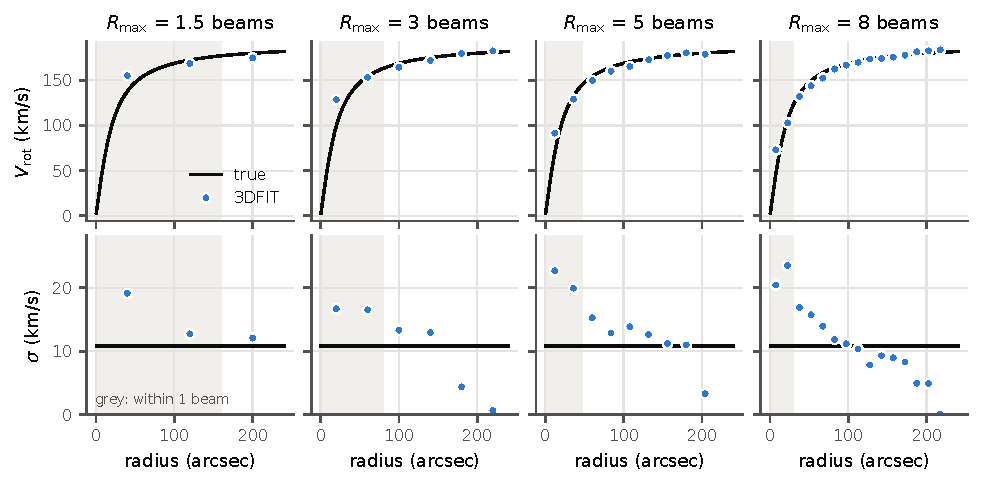
\includegraphics[width=\textwidth]{fig_examples}
\caption{One galaxy (the median $V_\mathrm{flat}$ of the sample) observed at the four spatial
resolutions, with $\dvs = 1$ and peak S/N = 20. Lines: true profiles; points: 3DFIT. The grey band is
the first beam.}
\label{fig:examples}
\end{figure}

\subsection{Spatial and spectral resolution}
Figure~\ref{fig:maps} and Table~\ref{tab:resolution} give the errors over the $4\times4$ grid at peak
S/N = 20.
\begin{itemize}
\item $\vrot$ is underestimated by 0--2\% when the disk is $\geq 3$ beams across and by 4--7\% at 1.5
  beams. The scatter decreases from 11--14\% at 1.5 beams to 6--7\% at 3 beams and 3--4\% at 5--8 beams
  (for $\dvs \leq 2$). Channels as wide as $4\sigma$ increase it to 6--11\%.
\item $\sigma$ is overestimated by 15--29\% at 1.5 beams and by 10--11\% at 3 beams (for $\dvs \leq 2$),
  and is unbiased within $\pm6$\% at 5 and 8 beams. Its scatter, 25--36\% for $\dvs \leq 2$ and 42--57\%
  for $\dvs = 4$, hardly depends on the spatial resolution: it is set by the S/N of the rings
  (Section~\ref{sec:snr}). Channels narrower than $\sigma$ improve the scatters only slightly.
\item 93--100\% of the rings are fitted; the missing ones are the faint outermost rings.
\end{itemize}
Figure~\ref{fig:sweeps} shows the same trends along the two axes through the reference configuration
for the four S/N values. The S/N matters more than the resolution: at peak S/N = 5, $\sigma$ is
underestimated by 43--64\% at every resolution and only 25--78\% of the rings are fitted, while the
scatter of $\vrot$ at 3 beams is 15\% at S/N 10 against 7\% at S/N 20.

\begin{figure}[tbp]
\centering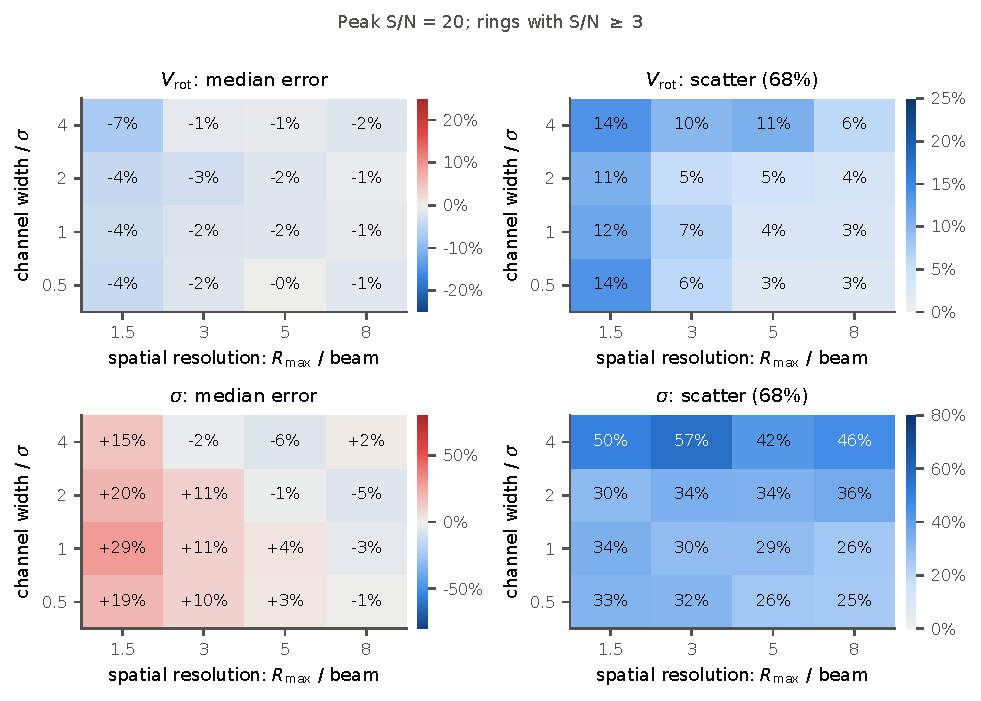
\includegraphics[width=0.92\textwidth]{fig_maps}
\caption{Median error (left) and scatter (right) of $\vrot$ (top) and $\sigma$ (bottom) as a function
of the spatial resolution (disk radius in beams) and of the channel width in units of the gas
dispersion, at peak S/N = 20 (rings with S/N $\geq 3$). Red: overestimate; blue: underestimate.}
\label{fig:maps}
\end{figure}

\begin{table}[tbp]
\centering\small
\caption{Errors at peak S/N = 20 (rings with S/N $\geq 3$; 24 galaxies per row). ``Time'' is the
median duration of a fit (one thread).}
\label{tab:resolution}
\begin{tabular}{cc rr rr r r}
\toprule
 & & \multicolumn{2}{c}{$V_\mathrm{rot}$ error (\%)} & \multicolumn{2}{c}{$\sigma$ error (\%)} & rings & time \\
$R_\mathrm{max}$/beam & $\Delta v/\sigma$ & median & scatter & median & scatter & fitted (\%) & (s) \\
\midrule
1.5 & 0.5 & $-$4.1 & 13.6 & +19.4 & 32.5 & 100 & 0.1 \\
1.5 & 1 & $-$3.7 & 11.7 & +28.9 & 33.9 & 100 & 0.1 \\
1.5 & 2 & $-$4.1 & 10.6 & +20.2 & 30.4 & 100 & 0.1 \\
1.5 & 4 & $-$7.0 & 13.6 & +15.0 & 50.1 & 100 & 0.1 \\
\addlinespace
3 & 0.5 & $-$1.9 & 6.1 & +10.2 & 32.1 & 99 & 0.3 \\
3 & 1 & $-$2.0 & 6.8 & +10.6 & 29.5 & 100 & 0.2 \\
3 & 2 & $-$3.2 & 5.4 & +10.7 & 34.3 & 100 & 0.1 \\
3 & 4 & $-$1.0 & 9.8 & $-$2.2 & 56.6 & 99 & 0.1 \\
\addlinespace
5 & 0.5 & $-$0.4 & 2.5 & +3.0 & 25.6 & 96 & 1.1 \\
5 & 1 & $-$1.6 & 3.6 & +4.1 & 29.4 & 96 & 0.7 \\
5 & 2 & $-$1.6 & 4.5 & $-$1.4 & 33.7 & 97 & 0.4 \\
5 & 4 & $-$0.8 & 10.6 & $-$6.2 & 42.0 & 99 & 0.3 \\
\addlinespace
8 & 0.5 & $-$1.4 & 2.5 & $-$0.7 & 24.9 & 93 & 2.4 \\
8 & 1 & $-$0.8 & 3.3 & $-$3.2 & 25.8 & 94 & 1.4 \\
8 & 2 & $-$0.7 & 3.6 & $-$5.2 & 35.9 & 96 & 1.1 \\
8 & 4 & $-$1.8 & 6.0 & +1.7 & 45.6 & 95 & 0.8 \\
\bottomrule
\end{tabular}

\end{table}

\begin{figure}[tbp]
\centering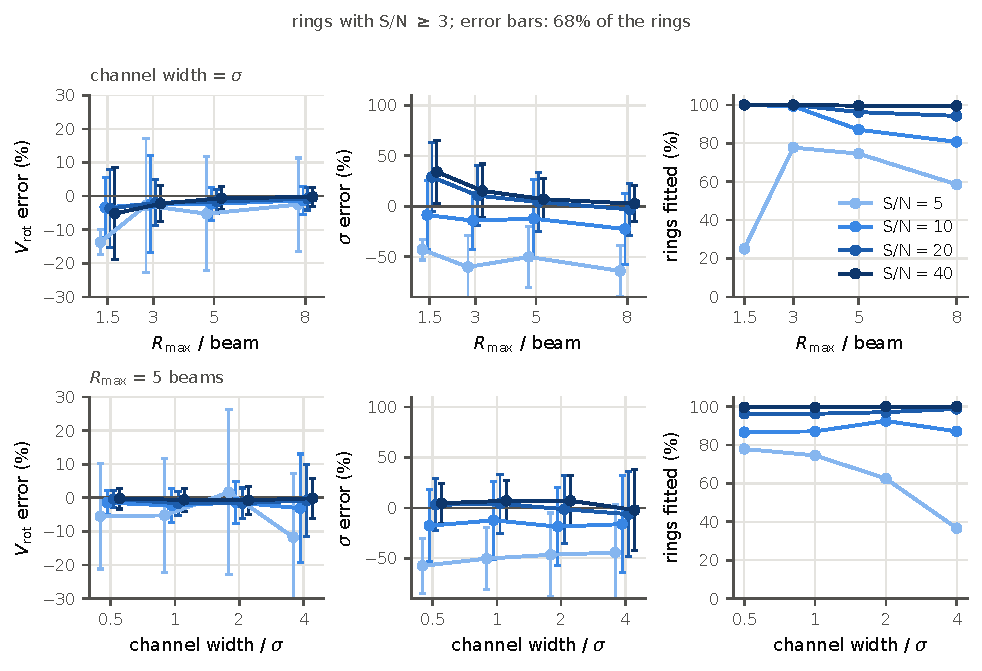
\includegraphics[width=\textwidth]{fig_sweeps}
\caption{Errors along the spatial (top) and spectral (bottom) axes through the reference configuration,
for the four peak S/N values (symbols slightly offset for clarity). Error bars: 16--84\% of the rings.
Right: percentage of the rings fitted (failed fits count as zero).}
\label{fig:sweeps}
\end{figure}

\subsection{Signal-to-noise ratio}\label{sec:snr}
At the reference resolution (Table~\ref{tab:snr}) the median error of $\vrot$ goes from $-5$\% at peak
S/N = 5 to $-0.6$\% at 40 and the scatter from 17\% to 3--4\% (5\% at S/N 10). Nearly 90\% of the rings
have $\vrot$ within 10\% of the truth from S/N 10 up. The dispersion behaves very differently: its
median error rises monotonically with the S/N, from $-50$\% to $+7$\%, and only 43--62\% of the rings
have $\sigma$ within 20\% from S/N 10 up.

\begin{table}[tbp]
\centering\small
\caption{Errors at the reference resolution ($N_b = 5$, $\dvs = 1$) as a function of the peak S/N
(rings with S/N $\geq 3$). ``Within'': fraction of the rings with $|$error$|$ below 10\% ($\vrot$) and
20\% ($\sigma$).}
\label{tab:snr}
\begin{tabular}{r rr rr rr r}
\toprule
 & \multicolumn{2}{c}{$V_\mathrm{rot}$ error (\%)} & \multicolumn{2}{c}{$\sigma$ error (\%)} & \multicolumn{2}{c}{within 10\% / 20\%} & failed \\
peak S/N & median & scatter & median & scatter & $V_\mathrm{rot}$ & $\sigma$ & fits \\
\midrule
5 & $-$5.2 & 16.9 & $-$50.3 & 30.4 & 45\% & 14\% & 0/24 \\
10 & $-$2.3 & 5.0 & $-$12.3 & 38.4 & 86\% & 43\% & 0/24 \\
20 & $-$1.6 & 3.6 & +4.1 & 29.4 & 89\% & 50\% & 0/24 \\
40 & $-$0.6 & 3.4 & +7.0 & 20.3 & 89\% & 62\% & 0/24 \\
\bottomrule
\end{tabular}

\end{table}

The S/N of the individual rings explains this (Figure~\ref{fig:ringsnr}). $\vrot$ is unbiased down to a
ring S/N of about 3 and fails below 2. $\sigma$ is underestimated by about 20\% at a ring S/N of 6,
by 50--65\% at 4 and by 75--90\% below 3, nearly independently of the channel width; it is unbiased at
S/N $\approx 10$ and \emph{over}estimated, by 10--25\%, at S/N 15--30. The two effects are explained in
Section~\ref{sec:origin}: the mask at low S/N and the normalisation of the ring models at high S/N.

\begin{figure}[tbp]
\centering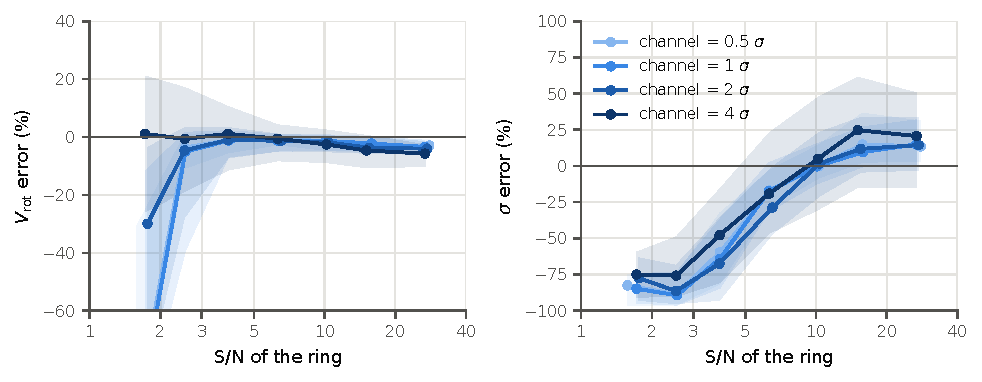
\includegraphics[width=\textwidth]{fig_ringsnr}
\caption{Error of each ring against its own S/N, for all the configurations of the resolution
experiment and the four channel widths (rings beyond one beam from the centre). Lines: median;
bands: 16--84\%.}
\label{fig:ringsnr}
\end{figure}

\subsection{Radial trends: beam smearing}
Figure~\ref{fig:radius} shows the errors against radius in beams (peak S/N 20 and 40, rings with S/N
$\geq3$). In the innermost ring (the first half beam) $\vrot$ is overestimated by 15--100\% (the true
velocity is small there), and between one and two beams it is underestimated by 1--7\%; beyond three
beams it is unbiased. $\sigma$ is overestimated by 10--45\% within two beams of the centre, where the rotation
curve rises and the line profiles of the data are broadened by the unresolved velocity gradient
(3DFIT convolves the model with the beam, but each ring is modelled alone, without the emission of the
rings around it), and underestimated in the outermost rings, where the S/N is low.

\begin{figure}[tbp]
\centering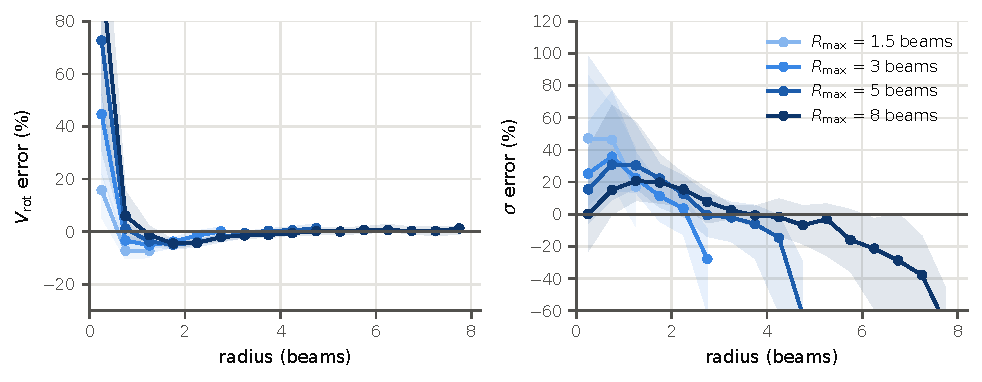
\includegraphics[width=\textwidth]{fig_radius}
\caption{Errors against radius in beams for the four spatial resolutions ($\dvs = 1$, peak S/N 20 and 40,
rings with S/N $\geq3$). Lines: median; bands: 16--84\%.}
\label{fig:radius}
\end{figure}

%======================================================================
\section{Geometry and kinematics}\label{sec:geometry}
%======================================================================

\subsection{Flat disks}
Table~\ref{tab:geometry} and Figure~\ref{fig:geometry} summarise the 200 flat disks fitted with INC and
PA free.
\begin{itemize}
\item The position angle is recovered with a scatter of 1.5--3$^\circ$ and no bias at any inclination
  (and $\lesssim 1^\circ$ at S/N 40); a few low-S/N face-on disks are off by 10$^\circ$.
\item The inclination is biased at both ends: by $+8^\circ$ at 15--30$^\circ$ (scatter $13^\circ$) and by
  $-7^\circ$ at 75--86$^\circ$. Between 30 and 75$^\circ$ the error is \GeoDefIncMed$\pm$\GeoDefIncSig$^\circ$
  (\GeoDefWithin\% of the galaxies within $3^\circ$), and the scatter decreases with inclination, from
  $10^\circ$ at 30--45$^\circ$ to $3^\circ$ at 60--75$^\circ$.
\item The errors of $\vrot$ follow those of INC ($\vrot \propto 1/\sin i$): $-33$\% at 15--30$^\circ$,
  $-5$ to $-7$\% at 30--60$^\circ$ and $-1$ to $-3$\% above $60^\circ$ (rings beyond $0.3\,\rmax$).
  The scatter of $\vrot$ at 30--75$^\circ$ is \GeoDefVSig\% (against 3.6\% with the geometry known).
\item $\sigma$ follows the S/N as with fixed geometry (Figure~\ref{fig:geometry}, bottom right), and is
  overestimated at the highest inclinations.
\end{itemize}

\begin{table}[tbp]
\centering\small
\caption{Flat disks with INC and PA free: errors by true inclination for the three fit modes. For each
galaxy the median over its rings is taken ($\vrot$: rings beyond $0.3\,\rmax$); the table gives the
median and scatter over the galaxies (all S/N values together).}
\label{tab:geometry}
\begin{tabular}{l l r rr rr rr}
\toprule
 & & & \multicolumn{2}{c}{INC error ($^\circ$)} & \multicolumn{2}{c}{PA error ($^\circ$)} & $V_\mathrm{rot}$ & $\sigma$ \\
limits & INC range & fits & median & scatter & median & scatter & error (\%) & error (\%) \\
\midrule
estimates, default limits & 15--30$^\circ$ & 44 & +8.2 & 13.2 & +0.3 & 2.7 & $-$32.8 & $-$27.2 \\
estimates, default limits & 30--45$^\circ$ & 43 & +2.3 & 10.3 & +0.7 & 2.7 & $-$6.7 & $-$18.0 \\
estimates, default limits & 45--60$^\circ$ & 46 & +2.6 & 6.0 & +0.1 & 1.5 & $-$5.1 & $-$11.5 \\
estimates, default limits & 60--75$^\circ$ & 41 & +0.6 & 2.9 & +0.1 & 2.3 & $-$2.9 & $-$7.9 \\
estimates, default limits & 75--86$^\circ$ & 26 & $-$6.7 & 4.4 & $-$0.0 & 1.6 & $-$1.2 & +11.0 \\
\addlinespace
estimates, wide limits & 15--30$^\circ$ & 44 & +8.5 & 14.2 & +0.3 & 2.9 & $-$32.8 & $-$31.2 \\
estimates, wide limits & 30--45$^\circ$ & 43 & +1.7 & 10.0 & +1.0 & 2.6 & $-$6.4 & $-$20.2 \\
estimates, wide limits & 45--60$^\circ$ & 46 & +3.0 & 6.0 & $-$0.1 & 1.6 & $-$5.3 & $-$18.3 \\
estimates, wide limits & 60--75$^\circ$ & 41 & +0.6 & 5.2 & +0.1 & 2.3 & $-$2.0 & $-$7.6 \\
estimates, wide limits & 75--86$^\circ$ & 26 & $-$6.7 & 5.1 & $-$0.2 & 1.0 & $-$0.8 & +9.5 \\
\addlinespace
true values, default limits & 15--30$^\circ$ & 44 & +1.3 & 1.5 & +0.6 & 4.1 & $-$10.2 & $-$33.1 \\
true values, default limits & 30--45$^\circ$ & 43 & +2.2 & 2.0 & +0.2 & 2.6 & $-$7.7 & $-$17.5 \\
true values, default limits & 45--60$^\circ$ & 46 & +1.9 & 3.9 & +0.1 & 1.2 & $-$3.6 & $-$8.9 \\
true values, default limits & 60--75$^\circ$ & 41 & +0.8 & 4.4 & +0.1 & 1.7 & $-$2.4 & $-$10.9 \\
true values, default limits & 75--86$^\circ$ & 26 & +1.0 & 3.5 & +0.4 & 1.3 & $-$1.3 & +1.1 \\
\bottomrule
\end{tabular}

\end{table}

\begin{figure}[tbp]
\centering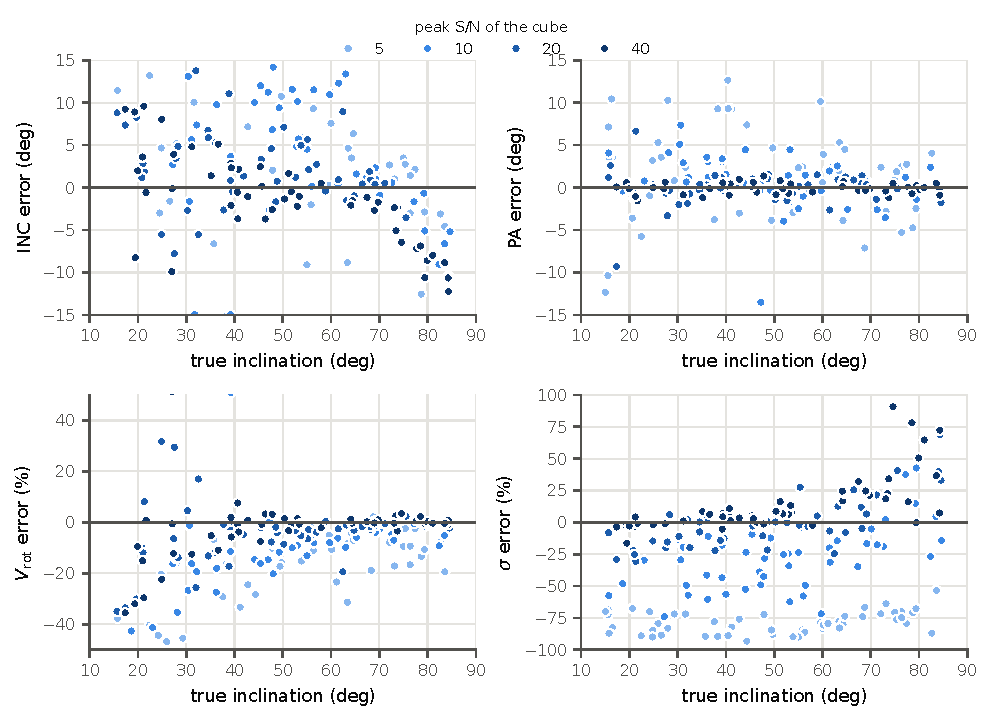
\includegraphics[width=\textwidth]{fig_geometry}
\caption{Flat disks fitted from the estimated INC and PA with the default limits: errors (median over the
rings of each galaxy) against the true inclination, coloured by the peak S/N of the cube.}
\label{fig:geometry}
\end{figure}

Table~\ref{tab:geometry_snr} splits the galaxies with 30--75$^\circ$ by S/N. With the default fit the INC
error is $+3.5\pm9.9^\circ$ at S/N 5, $+4.5\pm6.9^\circ$ at 10, $+1.2\pm3.6^\circ$ at 20 and
$-1.2\pm2.4^\circ$ at 40: the scatter decreases with the S/N, but the bias changes sign. When the fit
starts from the true INC and PA the scatter becomes small (0.5--2.5$^\circ$), which shows that most of
the scatter of the default fits comes from the initial estimates (next section), but the S/N-dependent
bias remains: from $+4.8^\circ$ at S/N 5 (at the $+5^\circ$ limit of DELTAINC) to $-3.1^\circ$ at S/N 40.
This bias is a property of 3DFIT, discussed in Section~\ref{sec:origin}.

\begin{table}[tbp]
\centering\small
\caption{Flat disks with true inclination 30--75$^\circ$, by peak S/N.}
\label{tab:geometry_snr}
\begin{tabular}{l r r rr rr rr}
\toprule
 & & & \multicolumn{2}{c}{INC error ($^\circ$)} & \multicolumn{2}{c}{PA error ($^\circ$)} & $V_\mathrm{rot}$ & $\sigma$ \\
initial INC, PA & S/N & fits & median & scatter & median & scatter & error (\%) & error (\%) \\
\midrule
estimates, default limits & 5 & 29 & +3.5 & 9.9 & +2.3 & 6.1 & $-$15.1 & $-$80.6 \\
estimates, default limits & 10 & 39 & +4.5 & 6.9 & +0.7 & 2.4 & $-$6.2 & $-$25.3 \\
estimates, default limits & 20 & 31 & +1.2 & 3.6 & +0.3 & 1.4 & $-$2.9 & $-$0.5 \\
estimates, default limits & 40 & 31 & $-$1.2 & 2.4 & +0.1 & 0.7 & $-$0.3 & +8.0 \\
\addlinespace
estimates, wide limits & 5 & 29 & +6.9 & 9.5 & +2.7 & 7.0 & $-$15.2 & $-$74.6 \\
estimates, wide limits & 10 & 39 & +4.6 & 5.8 & +0.8 & 2.4 & $-$7.4 & $-$29.2 \\
estimates, wide limits & 20 & 31 & +1.2 & 3.5 & $-$0.0 & 1.0 & $-$1.2 & $-$2.1 \\
estimates, wide limits & 40 & 31 & $-$1.2 & 2.4 & +0.4 & 0.6 & +1.2 & +6.6 \\
\addlinespace
true values, default limits & 5 & 29 & +4.8 & 0.5 & +2.2 & 4.5 & $-$11.2 & $-$81.8 \\
true values, default limits & 10 & 39 & +3.4 & 1.5 & +0.2 & 2.1 & $-$6.1 & $-$27.6 \\
true values, default limits & 20 & 31 & +0.3 & 1.7 & $-$0.1 & 0.7 & $-$2.3 & $-$2.3 \\
true values, default limits & 40 & 31 & $-$3.1 & 2.5 & $-$0.0 & 0.8 & +1.4 & +7.0 \\
\bottomrule
\end{tabular}

\end{table}

\subsection{The role of the initial estimates}
3DFIT does not move the inclination far from where it starts (Figure~\ref{fig:geometry_init}). The
final errors correlate with the errors of the initial estimate with coefficient \GeoDefCorr{}
(30--75$^\circ$); the median change of INC during the fit is \GeoDefMove$^\circ$, and 20\% of the fits end
within $0.5^\circ$ of the $\pm5^\circ$ limit. The initial estimates of BBarolo (from the moment maps) are good for the
position angle (median error $0.5$--$1.6^\circ$) but biased for the inclination: by $+7^\circ$ at
15--30$^\circ$, $+3$ to $+4^\circ$ at 30--60$^\circ$, $+1.5^\circ$ at 60--75$^\circ$ and $-7^\circ$ above
75$^\circ$, with a scatter of $10$--$12^\circ$ below 45$^\circ$. These biases go directly into the fit.
Widening the limits to DELTAINC = $15^\circ$ and DELTAPA = $30^\circ$ does not help: the INC scatter
grows from \GeoDefIncSig{} to \GeoWideIncSig$^\circ$ and the correlation with the estimate stays high
(\GeoWideCorr): the minimum of the residuals in INC is shallow, and the fit drifts rather than converging
to the true value.

\begin{figure}[tbp]
\centering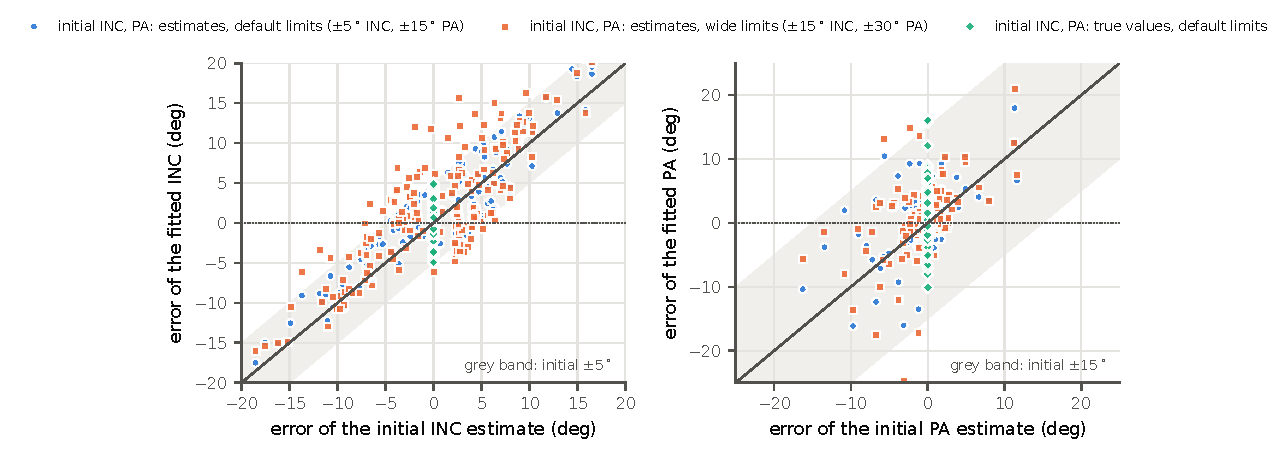
\includegraphics[width=\textwidth]{fig_geometry_init}
\caption{Error of the fitted INC (left) and PA (right) against the error of the initial value, for the
three fit modes (median over the rings of each galaxy). The diagonal is ``no improvement''; the grey band
is the default DELTAINC (DELTAPA) window. The ``true values'' fits start at zero.}
\label{fig:geometry_init}
\end{figure}

\subsection{Warped disks}
For the 120 warped disks (peak S/N 20), the errors averaged over the rings are similar to those of the
flat disks (Table~\ref{tab:warp}: INC \WarpDefIncMed$\pm$\WarpDefIncSig$^\circ$, PA scatter
\WarpDefPASig$^\circ$), but these averages are dominated by the inner flat disk. The warp itself is
recovered only in position angle (Figures~\ref{fig:warp_examples} and~\ref{fig:warp_amp}): the change of
PA between the inner disk and the outer rings is recovered with a slope of \WarpDefPASlope{} (fitted
against true), while the fitted change of INC does not correlate with the true one (slope
\WarpDefIncSlope; \WarpWideIncSlope{} with the wide limits). 3DFIT starts from a single estimated
inclination; the stage-1 inclinations of the outer rings can move only $5^\circ$ from it and are noisy,
and the regularisation (a constant when the stage-1 values scatter by less than 3$^\circ$) flattens what
is left. Starting from the true profiles, 70\% of the INC warp (slope \WarpTrueIncSlope) and 77\% of the
PA warp are kept, the rest being lost to the regularisation and to the limits. Figure~\ref{fig:warp_cdf}
compares the distributions of the ring errors of the flat and warped disks.

\begin{table}[tbp]
\centering\small
\caption{Warped disks (peak S/N 20): errors by fit mode (median over the rings of each galaxy, then over the
galaxies).}
\label{tab:warp}
\begin{tabular}{l l r rr rr rr}
\toprule
 & & & \multicolumn{2}{c}{INC error ($^\circ$)} & \multicolumn{2}{c}{PA error ($^\circ$)} & $V_\mathrm{rot}$ & $\sigma$ \\
limits & INC range & fits & median & scatter & median & scatter & error (\%) & error (\%) \\
\midrule
estimates, default limits & all & 120 & +0.0 & 5.0 & +0.2 & 1.8 & $-$1.9 & +2.5 \\
\addlinespace
estimates, wide limits & all & 120 & +0.2 & 4.3 & +0.1 & 1.9 & $-$0.9 & +1.0 \\
\addlinespace
true values, default limits & all & 120 & $-$0.3 & 2.0 & +0.2 & 1.8 & $-$1.1 & +4.4 \\
\bottomrule
\end{tabular}

\end{table}

\begin{figure}[tbp]
\centering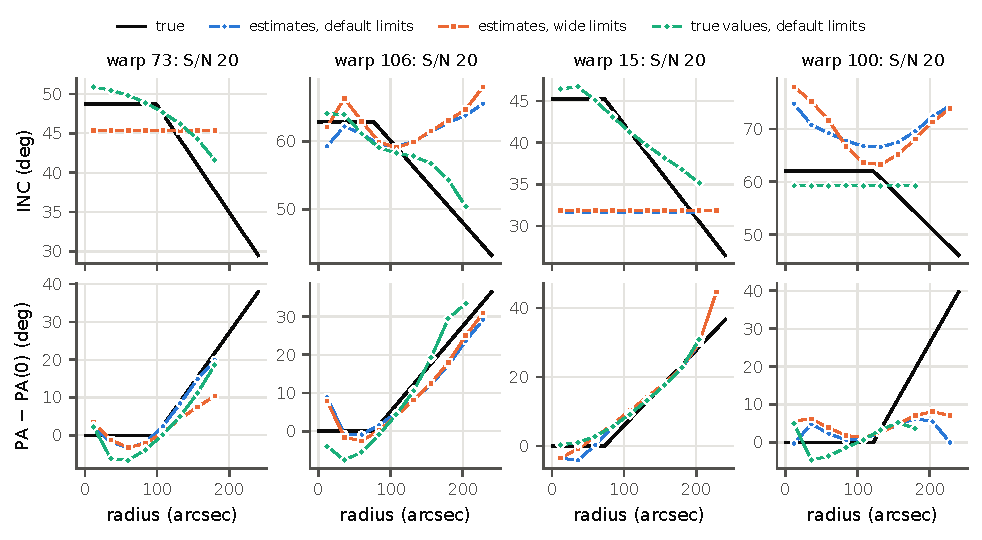
\includegraphics[width=\textwidth]{fig_warp_examples}
\caption{The four warped disks with the largest warps: true INC and PA profiles (black) and the fits in the
three modes.}
\label{fig:warp_examples}
\end{figure}

\begin{figure}[tbp]
\centering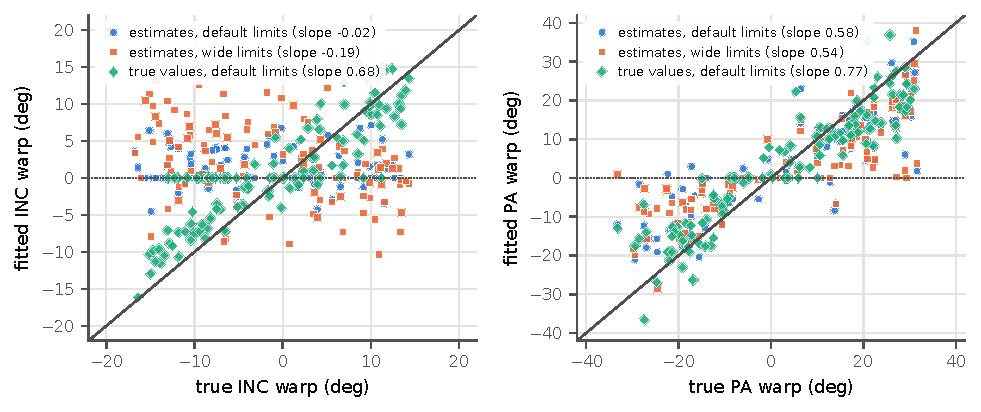
\includegraphics[width=\textwidth]{fig_warp_amp}
\caption{Fitted against true amplitude of the warps: change of INC (left) and PA (right) between the inner
flat disk and the two outermost rings. The slopes of linear fits are in the legends.}
\label{fig:warp_amp}
\end{figure}

\begin{figure}[tbp]
\centering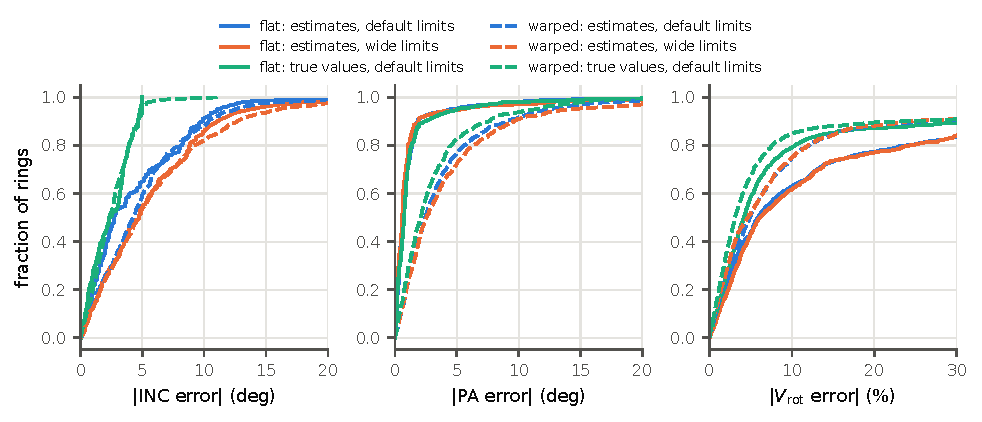
\includegraphics[width=\textwidth]{fig_warp_cdf}
\caption{Cumulative distributions of the absolute errors of all the rings of the flat (solid; peak S/N
$\geq 20$) and warped (dashed; S/N 20) disks, for the three fit modes.}
\label{fig:warp_cdf}
\end{figure}

%======================================================================
\section{Origin of the systematic errors}\label{sec:origin}
%======================================================================

Two errors depend on the S/N in opposite directions: $\sigma$ goes from underestimated at low S/N to
overestimated at high S/N, and INC (with the fit started at the true value) from overestimated to
underestimated. Since the C++ BBarolo shows the same trends on the same cubes
(Section~\ref{sec:cpp}), they are properties of the algorithm, not of the port. We traced them with the
additional fits of the ``mask'' and ``diagnostic'' experiments.

\subsection{Low S/N: the mask}
In the residuals of a ring, a voxel outside the mask where the model has flux is a ``blank'': its
residual is added to the sum, but the sum is divided by the number of voxels \emph{inside} the mask and
then multiplied by $(1 + N_\mathrm{blank}/N_\mathrm{tot})^\mathrm{BWEIGHT}$. Model flux outside the mask
is therefore penalised, also with BWEIGHT = 0. At low S/N the mask built by the source finder (MASK =
SEARCH) keeps only the bright cores of the line profiles and of the disk, so the fit prefers narrower
lines (smaller $\sigma$) and a thinner projected disk (larger INC). Table~\ref{tab:mask} and Figure~\ref{fig:mask} show
the evidence, on the same cubes:
\begin{itemize}
\item with MASK = SMOOTH\&SEARCH, which includes fainter emission, the $\sigma$ bias at S/N 5 decreases
  from \MaskSearchFiveS{} to \MaskSmoothFiveS\% and the INC bias at S/N 10 from \MaskSearchTenInc{} to
  \MaskSmoothTenInc$^\circ$;
\item with BWEIGHT = 0 (no extra weight for the blanks) the $\sigma$ bias at S/N 10 disappears
  (\MaskNoblankTenS\%), but not at S/N 5 (\MaskNoblankFiveS\%);
\item without mask (MASK = NONE) the INC bias at S/N 5 disappears (\MaskNoneFiveInc$^\circ$); this is not
  a usable option, though: the residuals replace the data values below zero with the noise level, so
  the noise acquires a positive pedestal that the fit reproduces with very broad lines ($\sigma$
  overestimated by \MaskNoneFortyS\% even at S/N 40, by \MaskNoneFiveS\% at S/N 5).
\end{itemize}

\begin{table}[tbp]
\centering\small
\caption{The same cubes fitted with other options: the reference configuration with fixed geometry
(rings with S/N $\geq 3$) and the flat disks with 30--75$^\circ$ fitted from the true INC and PA (default
limits). ``Defaults'': MASK = SEARCH, BWEIGHT = 1, NORM = AZIM.}
\label{tab:mask}
\begin{tabular}{l r rr rr rr r}
\toprule
 & & \multicolumn{2}{c}{$V_\mathrm{rot}$ error (\%)} & \multicolumn{2}{c}{$\sigma$ error (\%)} & \multicolumn{2}{c}{INC error ($^\circ$)} & failed \\
 & & \multicolumn{4}{c}{fixed geometry} & \multicolumn{2}{c}{flat disks} & fits \\
\cmidrule(lr){3-6}\cmidrule(lr){7-8}
3DFIT options & peak S/N & median & scatter & median & scatter & median & scatter & \\
\midrule
defaults & 5 & $-$5.2 & 16.9 & $-$50.3 & 30.4 & +4.8 & 0.5 & 0/53 \\
 & 10 & $-$2.3 & 5.0 & $-$12.3 & 38.4 & +3.4 & 1.5 & 0/63 \\
 & 20 & $-$1.6 & 3.6 & +4.1 & 29.4 & +0.3 & 1.7 & 0/55 \\
 & 40 & $-$0.6 & 3.4 & +7.0 & 20.3 & $-$3.1 & 2.5 & 0/55 \\
\addlinespace
MASK = SMOOTH\&SEARCH & 5 & $-$3.9 & 16.2 & $-$30.9 & 32.1 & +4.6 & 0.5 & 2/53 \\
 & 10 & $-$2.2 & 5.0 & $-$8.6 & 39.4 & +1.1 & 1.6 & 0/63 \\
 & 20 & $-$0.9 & 4.2 & +1.9 & 29.7 & $-$1.1 & 2.5 & 0/55 \\
 & 40 & $-$0.1 & 3.9 & +4.1 & 22.7 & $-$3.7 & 1.9 & 0/55 \\
\addlinespace
MASK = NONE & 5 & $-$1.0 & 58.6 & +737.0 & 818.6 & +0.4 & 1.7 & 0/53 \\
 & 10 & $-$2.0 & 8.8 & +69.4 & 45.5 & $-$1.3 & 2.3 & 0/63 \\
 & 20 & $-$1.7 & 5.8 & +46.7 & 29.9 & $-$3.8 & 2.2 & 0/55 \\
 & 40 & $-$0.6 & 4.8 & +35.9 & 24.4 & $-$4.2 & 1.7 & 0/55 \\
\addlinespace
BWEIGHT = 0 & 5 & $-$4.2 & 16.8 & $-$44.5 & 31.3 & +4.7 & 0.6 & 0/53 \\
 & 10 & $-$2.1 & 4.6 & $-$1.8 & 33.3 & +3.1 & 1.6 & 0/63 \\
 & 20 & $-$1.0 & 3.7 & +9.3 & 28.1 & $-$0.4 & 2.3 & 0/55 \\
 & 40 & $-$0.4 & 3.6 & +12.3 & 19.6 & $-$2.7 & 2.0 & 0/55 \\
\addlinespace
NORM = LOCAL & 5 & $-$3.4 & 21.1 & $-$71.4 & 29.1 & +4.4 & 1.3 & 0/53 \\
 & 10 & $-$1.6 & 5.1 & $-$30.2 & 37.0 & +4.3 & 0.7 & 0/63 \\
 & 20 & $-$0.7 & 3.7 & $-$11.8 & 31.7 & +2.9 & 1.1 & 0/55 \\
 & 40 & $-$0.4 & 3.5 & $-$2.5 & 20.7 & +1.4 & 1.4 & 0/55 \\
\bottomrule
\end{tabular}

\end{table}

\begin{figure}[tbp]
\centering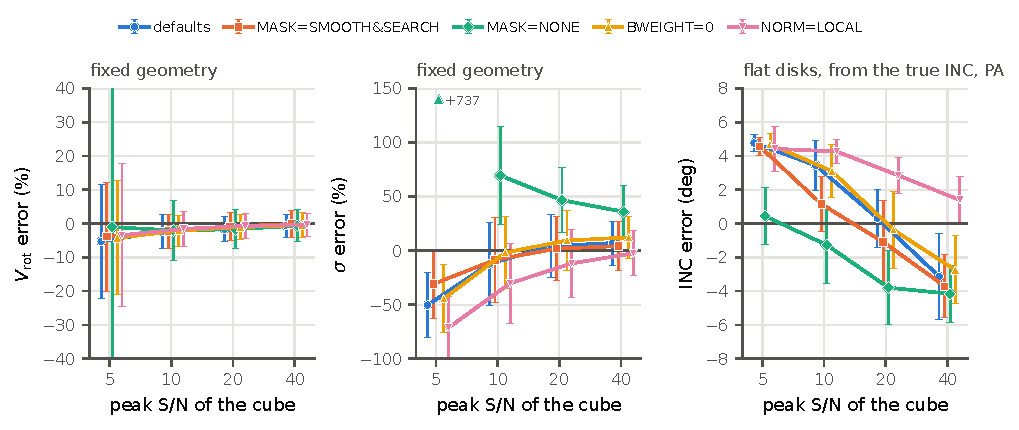
\includegraphics[width=\textwidth]{fig_mask}
\caption{Median errors against the peak S/N for the options of Table~\ref{tab:mask} (error bars:
16--84\%; symbols offset for clarity; the triangle marks a value off the scale).}
\label{fig:mask}
\end{figure}

\subsection{High S/N: the normalisation of single-ring models}\label{sec:azim}
At S/N 200, fitting six flat disks with INC = 45--75$^\circ$ from the true INC and PA but with DELTAINC =
$15^\circ$ (so that the minimum is not at the limit), the inclination is underestimated by
$\DiagDefault^\circ$ (median; $\sigma$ by $\DiagDefaultS$\%). The bias is in the function that 3DFIT
minimises: with $\vrot$, $\sigma$ and PA at their true values (and noise-free models), the residuals of a
single ring are smallest $\ScanHalf^\circ$ away from the true INC (Table~\ref{tab:incbias}). It does not come from the
simulations (it is the same for cubes made with the Monte-Carlo GALMOD, for razor-thin disks, and with
noise-free models in the fit), nor from the weighting function or the pixel sampling, and it does not
decrease with the number of beams across the disk. It decreases when the rings are wider than the beam
(rings one beam wide: $\DiagWide^\circ$; the minimum moves from $\ScanHalf^\circ$ to $\ScanTwo^\circ$ for
rings two beams wide), and it disappears when the normalisation is local (NORM = LOCAL:
$\DiagLocal^\circ$) or when the rest of the disk, at the true values, is added to the model of the ring
before the convolution ($\ScanRest^\circ$).

The interpretation: 3DFIT models each ring alone, convolved with the beam, and with NORM = AZIM rescales
it to the total flux of the data in the footprint of the ring. The data, though, also contain the
beam-smeared emission of the neighbouring rings. Near the minor axis of an inclined disk, a ring half a
beam wide projects to a strip much narrower than the beam ($b/2 \times \cos i$), and its smeared model is
fainter there, relative to the major axis, than the data. A lower inclination widens the projected ring
and moves model flux toward the minor axis, which reduces the residuals; broader lines ($\sigma$) do the
same in velocity. With a local normalisation the flux distribution does not enter the residuals, and
with the neighbouring rings in the model it is correct; reverse-cumulative fitting
(REVERSE = true), which adds the outer rings only, reduces the $\sigma$ bias but not the INC one.

NORM = LOCAL is not a complete remedy, however (Table~\ref{tab:mask}, Figure~\ref{fig:mask}): it removes
the high-S/N INC bias (\MaskLocalFortyInc$^\circ$ at S/N 40) but leaves the mask bias uncompensated
(\MaskLocalTenInc$^\circ$ at S/N 10, \MaskLocalTwentyInc$^\circ$ at 20), and it underestimates $\sigma$
more at every S/N. With the defaults, the two biases cancel near peak S/N 20, which is why the reference
configuration looks unbiased.

\begin{table}[tbp]
\centering\small
\caption{Inclination bias at S/N 200 (flat disks with INC = 45--75$^\circ$). A: 3DFIT fits from the true
INC and PA with DELTAINC = $15^\circ$ (six galaxies; median and range over the galaxies). B: position of
the minimum of the residual function of single rings (rings beyond $0.35\,\rmax$ of three galaxies), with
$\vrot$, $\sigma$ and PA at the true values and noise-free models (GALMODTYPE = ANALYTIC), scanned in steps
of $0.5^\circ$ from $-12^\circ$ to $+6^\circ$. Made by \code{diag\_incbias.py}.}
\label{tab:incbias}
\begin{tabular}{l rl r}
\toprule
 & \multicolumn{2}{c}{INC offset ($^\circ$)} & $\sigma$ error \\
test & median & [range] & (\%) \\
\midrule
\multicolumn{4}{l}{\emph{A. 3DFIT from the true INC and PA, DELTAINC = 15$^\circ$ (per galaxy: median over the rings)}} \\
as the geometry experiment & $-$7.3 & [$-$8.1, $-$5.7] & +14 \\
cube simulated with the Monte-Carlo GALMOD & $-$7.2 & [$-$8.7, $-$5.1] & +13 \\
razor-thin disk (Z0 = 0) & $-$6.3 & [$-$8.0, $-$3.7] & +13 \\
noise-free models in the fit (GALMODTYPE = ANALYTIC) & $-$7.1 & [$-$8.4, $-$5.2] & +17 \\
uniform azimuthal weights (WFUNC = 0) & $-$7.3 & [$-$8.9, $-$5.6] & +9 \\
local normalisation (NORM = LOCAL) & $-$1.3 & [$-$3.0, $-$0.3] & +7 \\
10 pixels per beam & $-$6.7 & [$-$7.9, $-$4.3] & +13 \\
disk radius = 12 beams & $-$8.4 & [$-$10.4, $-$7.3] & +5 \\
rings one beam wide & $-$3.4 & [$-$8.0, $-$0.5] & +7 \\
reverse-cumulative fit (REVERSE = true) & $-$6.5 & [$-$8.1, $-$4.7] & +8 \\
\addlinespace
\multicolumn{4}{l}{\emph{B. Minimum of the objective of single rings, other parameters at the true values (per ring)}} \\
ring alone, width = beam/2 (as 3DFIT) & $-$9.0 & [$-$12.0, $-$5.0] & \\
ring alone, width = beam & $-$8.0 & [$-$12.0, $-$4.0] & \\
ring alone, width = 2 beams & $-$5.0 & [$-$6.0, $-$4.5] & \\
ring alone, width = beam/2; uniform disk, flat rotation curve & $-$6.5 & [$-$12.0, +6.0] & \\
ring + rest of the disk (true values), width = beam/2 & $-$1.0 & [$-$5.0, +4.5] & \\
\bottomrule
\end{tabular}

\end{table}

%======================================================================
\section{Comparison with the C++ BBarolo}\label{sec:cpp}
%======================================================================

The C++ BBarolo 1.8 fitted the same cubes with the same parameters: the reference configuration at peak
S/N 10, 20 and 40 (\CppN{} rings with fixed geometry) and the \CppGeoN{} flat disks from the true INC and
PA. The two codes do not share the random numbers of the Monte-Carlo models, so they cannot agree ring
by ring better than the model noise allows. Figure~\ref{fig:cpp} and Table~\ref{tab:cpp} show that:
\begin{itemize}
\item with fixed geometry the Python $-$ C++ difference of $\vrot$ has median \CppVMed\% and scatter
  \CppVSig\%, smaller than the scatter of either code with respect to the truth (\CppVpySig{} and
  \CppVcppSig\%); for $\sigma$ the difference has median \CppSMed\% and scatter \CppSSig\%, and the median
  errors are \CppSpyMed\% (Python) and \CppScppMed\% (C++);
\item with INC and PA free, the fitted inclinations of a galaxy differ by \CppGeoDiff$^\circ$ (scatter;
  correlation \CppGeoCorr), and the S/N-dependent biases of INC, $\vrot$ and $\sigma$ are the same in the
  two codes (Table~\ref{tab:cpp}).
\end{itemize}
On these cubes a Python fit took \TimePyRes{}~s (fixed geometry) and \TimePyGeo{}~s (geometry, two
stages), median wall-clock time with one thread, against \TimeCppRes{} and \TimeCppGeo{}~s for the C++
executable. The C++ times include writing its standard outputs (model cubes, maps, PV diagrams), which the
Python fits of the suite skip, so this is not a like-for-like benchmark, but the pure-Python port is not
slower.

\begin{figure}[tbp]
\centering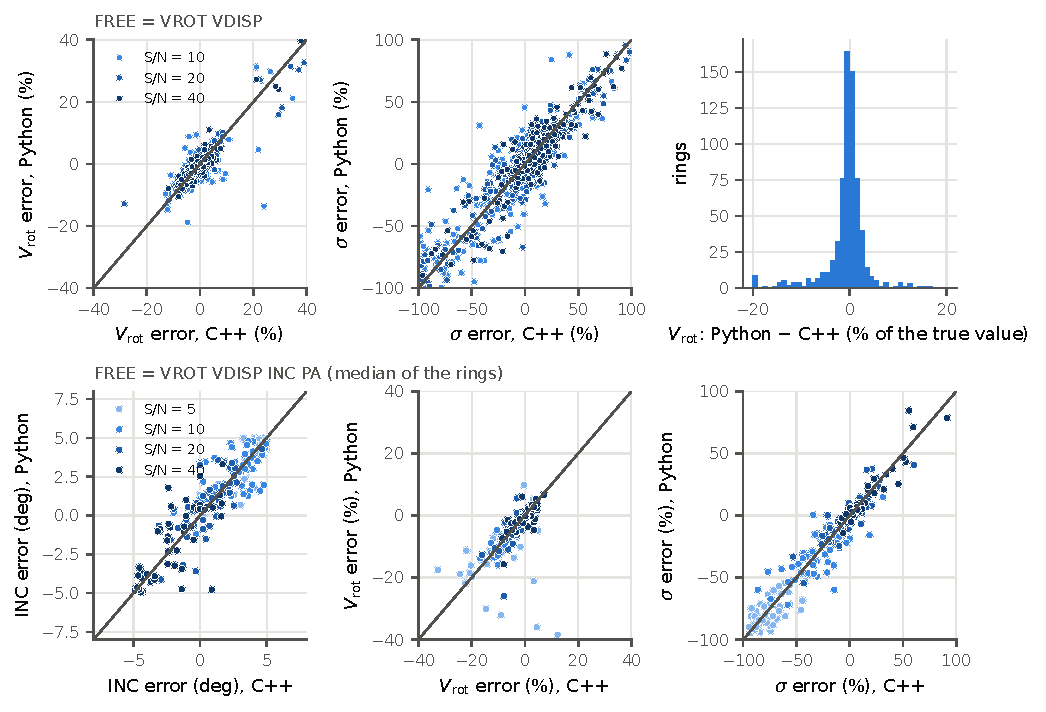
\includegraphics[width=\textwidth]{fig_cpp}
\caption{Python against C++ on the same cubes. Top: rings of the reference configuration with fixed
geometry, and the distribution of the Python $-$ C++ difference of $\vrot$. Bottom: flat disks fitted from
the true INC and PA (median over the rings of each galaxy).}
\label{fig:cpp}
\end{figure}

\begin{table}[tbp]
\centering\small
\caption{Flat disks with 30--75$^\circ$ fitted from the true INC and PA by the two codes (median over the
galaxies of the per-galaxy median errors).}
\label{tab:cpp}
\begin{tabular}{r r rr rr rr}
\toprule
 & & \multicolumn{2}{c}{INC error ($^\circ$)} & \multicolumn{2}{c}{$V_\mathrm{rot}$ error (\%)} & \multicolumn{2}{c}{$\sigma$ error (\%)} \\
S/N & galaxies & Python & C++ & Python & C++ & Python & C++ \\
\midrule
5 & 29 & +4.8 & +4.7 & $-$8.2 & $-$8.8 & $-$81.2 & $-$74.8 \\
10 & 39 & +3.4 & +3.4 & $-$5.9 & $-$5.8 & $-$27.6 & $-$21.3 \\
20 & 31 & +0.3 & +0.2 & $-$2.1 & $-$2.6 & $-$1.3 & +0.4 \\
40 & 31 & $-$3.1 & $-$2.5 & +0.7 & +1.6 & +7.0 & +10.0 \\
\bottomrule
\end{tabular}

\end{table}

%======================================================================
\section{Recommendations}\label{sec:recommendations}
%======================================================================

\paragraph{For the users of 3DFIT.}
\begin{itemize}
\item Trust $\vrot$ beyond the first half beam when the disk is at least 3 beams across and the rings
  have S/N $\gtrsim 3$; expect a scatter of 3--6\% per ring at $\geq5$ beams, 5--15\% at 3 beams and
  11--14\% at 1.5 beams, and a bias of a few \% within two beams of the centre.
\item Do not interpret the dispersion of rings with S/N $\lesssim 8$ (biased low), of the rings within two
  beams of the centre, or of disks less than 3 beams across (biased high). At low S/N, MASK =
  SMOOTH\&SEARCH reduces the bias. Never use MASK = NONE.
\item The fitted inclination is about as good as its initial value: provide a good one (e.g.\ from
  independent data or a careful 2DFIT), especially below 40$^\circ$ and above 75$^\circ$, where the
  automatic estimate is off by $\sim7^\circ$. Wider DELTAINC limits do not help.
\item At high S/N and INC $\gtrsim 45^\circ$, fit the geometry with rings at least one beam wide, or check
  the inclination with NORM = LOCAL: with the defaults it is underestimated by about $3^\circ$ at peak S/N 40
  and by up to $7^\circ$ at higher S/N.
\item For warps, provide a warped initial profile and check the regularisation (REGTYPE); from a single
  estimated inclination, 3DFIT does not find an inclination warp.
\end{itemize}

\paragraph{For the code.} Both systematics come from choices of the algorithm and could be removed:
\begin{itemize}
\item model each ring together with its neighbours (for example the current model of the other rings
  added before the convolution, as already done for REVERSE = true), or normalise the model of a ring
  with that of the whole disk;
\item treat the voxels outside the mask as unknown rather than as zero, or build the mask from the model
  (e.g.\ dilated), so that the low-S/N line wings do not bias $\sigma$ and INC;
\item revisit the automatic inclination estimate at the extremes, and the regularisation of the second
  stage for warps.
\end{itemize}
These changes would affect the C++ code as well; the tests of this suite can measure their effect.

\appendix
\sloppy
%======================================================================
\section{Running the suite}\label{app:run}
%======================================================================
The suite is in \code{pyBBarolo\_pure/performance}:
\begin{itemize}
\item \code{run\_suite.py} simulates and fits; one JSON line per fit is appended to
  \code{results/results.jsonl}, and an interrupted run continues where it stopped.\\
  \code{python run\_suite.py --outdir results --procs 8 [--cpp /path/to/BBarolo]}\\
  Options: \code{--experiments} (resolution, geometry, warp, cpp, mask), \code{--ngal} (24),
  \code{--ngeo} (200), \code{--nwarp} (120), \code{--seed} (2026), \code{--quick} (a few fits, to test the
  set-up). The cpp experiment runs only if a C++ executable is given (\code{--cpp} or
  \code{\$BBAROLO\_CPP}).
\item \code{diag\_incbias.py} runs the diagnostic of Section~\ref{sec:azim} (\code{--procs}, about five
  minutes with two processes).
\item \code{analyse.py} makes the figures (\code{report/figures}), tables (\code{report/tables}), the numbers
  quoted in the text (\code{report/numbers.tex}) and CSV files of all the fits and rings
  (\code{report/fits.csv}, \code{report/rings.csv}).
\item \code{cd report; pdflatex report; pdflatex report} builds this report.
\end{itemize}
The \NAll{} fits of this report took \TimeAll{} CPU minutes (simulation and fit, one thread per fit; less
than an hour with two processes); a fit with fixed geometry takes 0.1--2.5~s and one with INC and PA free
about 2~s.

%======================================================================
\section{Additional tables}\label{app:tables}
%======================================================================

\begin{table}[tbp]
\centering\small
\caption{As Table~\ref{tab:snr}, for all the fitted rings (no cut in ring S/N).}
\label{tab:snr_all}
\begin{tabular}{r rr rr rr r}
\toprule
 & \multicolumn{2}{c}{$V_\mathrm{rot}$ error (\%)} & \multicolumn{2}{c}{$\sigma$ error (\%)} & \multicolumn{2}{c}{within 10\% / 20\%} & failed \\
peak S/N & median & scatter & median & scatter & $V_\mathrm{rot}$ & $\sigma$ & fits \\
\midrule
5 & $-$8.4 & 28.3 & $-$72.1 & 28.2 & 44\% & 9\% & 0/24 \\
10 & $-$2.5 & 5.1 & $-$19.3 & 46.0 & 80\% & 38\% & 0/24 \\
20 & $-$1.6 & 3.8 & +1.6 & 31.6 & 88\% & 48\% & 0/24 \\
40 & $-$0.6 & 3.4 & +7.0 & 20.3 & 89\% & 62\% & 0/24 \\
\bottomrule
\end{tabular}

\end{table}

\end{document}
